\section{Opening a SQLite3 File Container}
\label{sec:sqlite_open}
For opening a file container, three actions are available:

\begin{itemize}  
\item New: Creates a new (empty) SQLite3 container and adds it to the 'File Selection' list
\item Add: Adds an existing  SQLite3 container and adds it to the 'File Selection' list
\item Remove: Removes an entry from the 'File Selection' list
\end{itemize}

After selection of the wanted database container, the 'Open' button can be used for opening the database container.

\begin{figure}[H]
  \center
    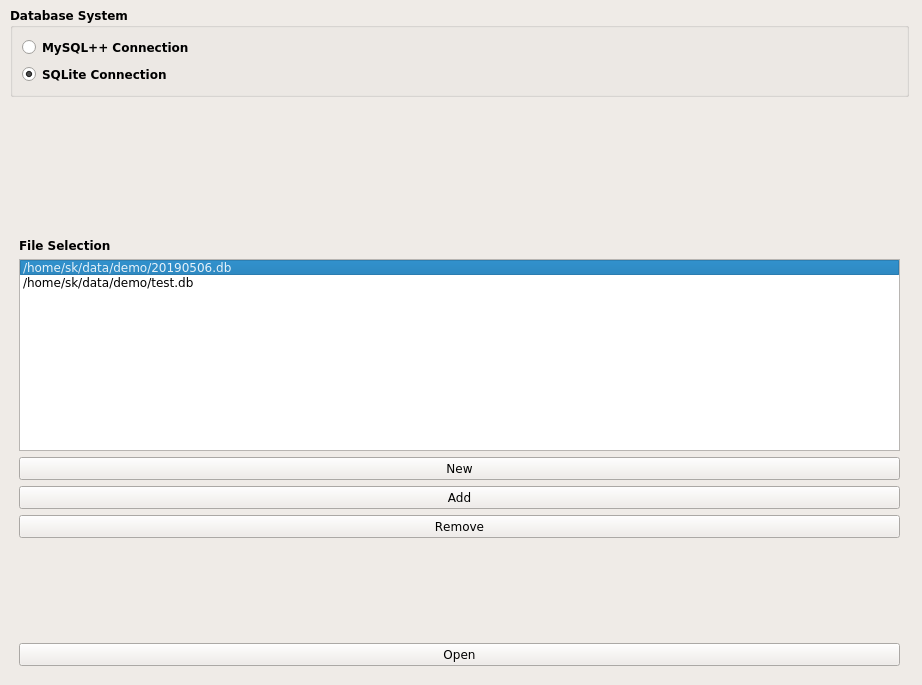
\includegraphics[width=8cm,frame]{../screenshots/sqlite3_open.png}
  \caption{Opening a SQLite3 file container}
  \label{fig:sqlite3_open}
\end{figure} 
